
%%%%%%%%%%%%%%%%%%%%%%%%%%%%%%%%%%%%%%%%%%%%%%%%%%%%%%%%%%%%%%%%%%%%%%%%%%%%%%%%
%
% Results
%
%%%%%%%%%%%%%%%%%%%%%%%%%%%%%%%%%%%%%%%%%%%%%%%%%%%%%%%%%%%%%%%%%%%%%%%%%%%%%%%%

\section{Results}
\label{sec:2lpt--results}

%%%%%%%%%%%%%%%%%%%%%%%%%%%%%%%%%%%%%%%%%%%%%%%%%%%%%%%%%%%%%%%%%%%%%%%%%%%%%%%%


With our catalog of matched dark matter halos, we directly compare differences in halo properties arising from initialization with \lpt\ vs \za.  We consider halos on a pair--by--pair basis as well as the entire sample as a whole.  Overall, we find \lpt\ halos undergo more growth at a given redshift than their \za\ counterparts.




%~~~~~~~~~~~~~~~~~~~~~~~~~~~~~~~~~~~~~~~~~~~~~~~~~~~~~~~~~~~~~~~~~~~~~~~~~~~~~~~
\subsection{Individual halo pairs}
%~~~~~~~~~~~~~~~~~~~~~~~~~~~~~~~~~~~~~~~~~~~~~~~~~~~~~~~~~~~~~~~~~~~~~~~~~~~~~~~


We compare large scale morphologies, density profiles, and various other halo properties for halo pairs on an individual halo--by--halo basis for several of the most massive halos.  Morphologies appear similar for most halos, indicating good halo matches between simulations.  However, many pairs display differences in central morphology, such as the number and separation of central density peaks.  We interpret these cases to be examples of differences in merger epochs, in which case one halo may still be undergoing a major merger, while its companion is in a more relaxed post-merger state.  We give an example of one such pair at $z = 6$ in Figure~\ref{fig:halo-pair}.  The top two rows show density projections of the nuclear regions for a large \lpt\ and matching \za\ halo (first and second rows, respectively).  We find  the \za\ halo to contain two distinct density peaks with a separation of $\sim 10$ kpc, while the \lpt\ halo displays only a single core.  On the third and fourth rows, we plot the density profiles of the same two halos (\lpt\ and \za, respectively).  Here, with nearly identical virial radii, it is readily seen that the \lpt\ halo is more concentrated than the \za\ halo.




%~~~~~~~~~~~~~~~~~~~~~~~~~~~~~~~~~~~~~~~~~~~~~~~~~~~~~~~~~~~~~~~~~~~~~~~~~~~~~~~
\subsection{Difference distributions of halo properties}
%~~~~~~~~~~~~~~~~~~~~~~~~~~~~~~~~~~~~~~~~~~~~~~~~~~~~~~~~~~~~~~~~~~~~~~~~~~~~~~~


\begin{figure*}[t]
	\centering
	\begin{subfigure}{}
		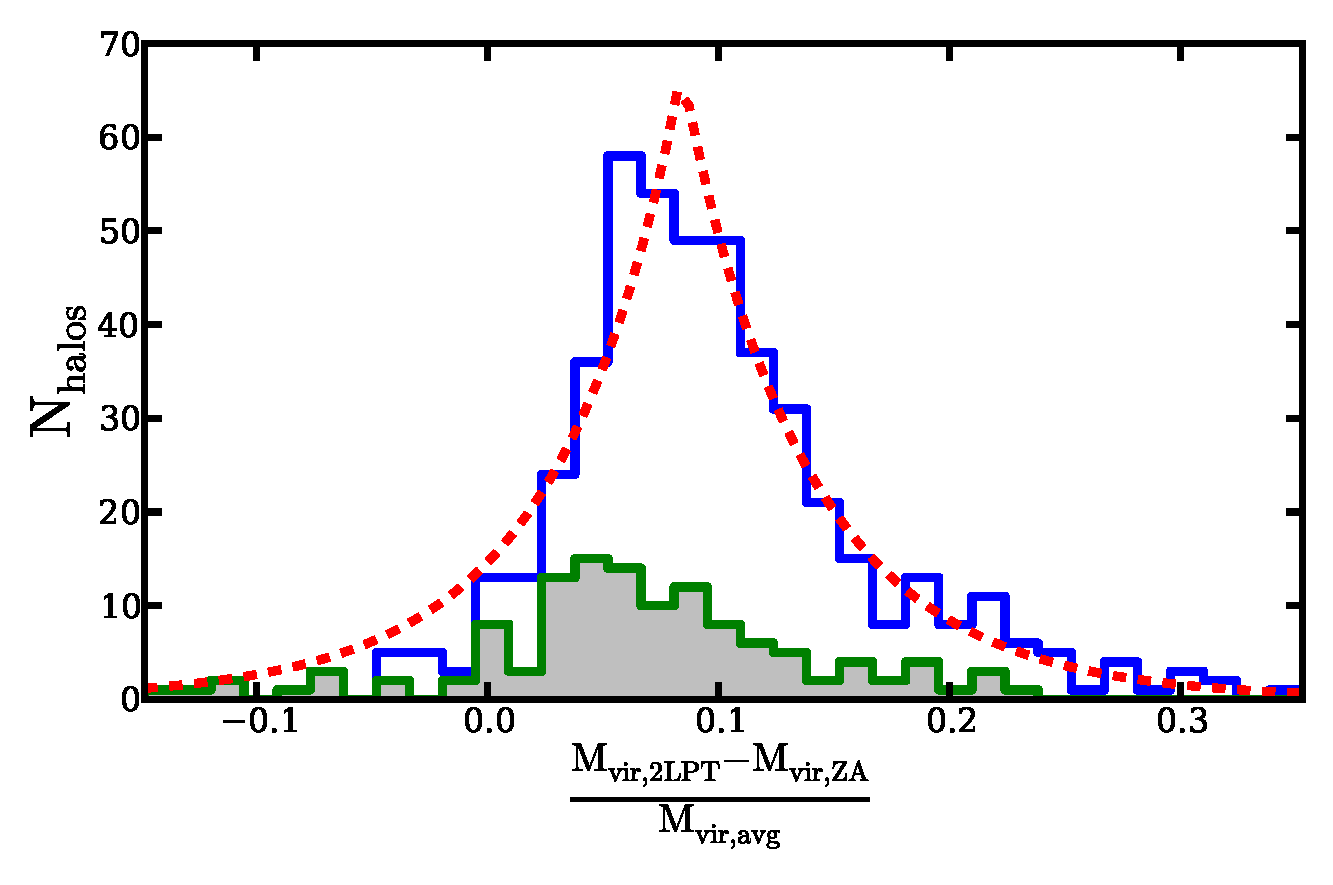
\includegraphics[width=0.48\linewidth]{diff-hist_Mvir_snap040_(0.0-1.0).eps}
	\end{subfigure}
	~
	\begin{subfigure}{}
		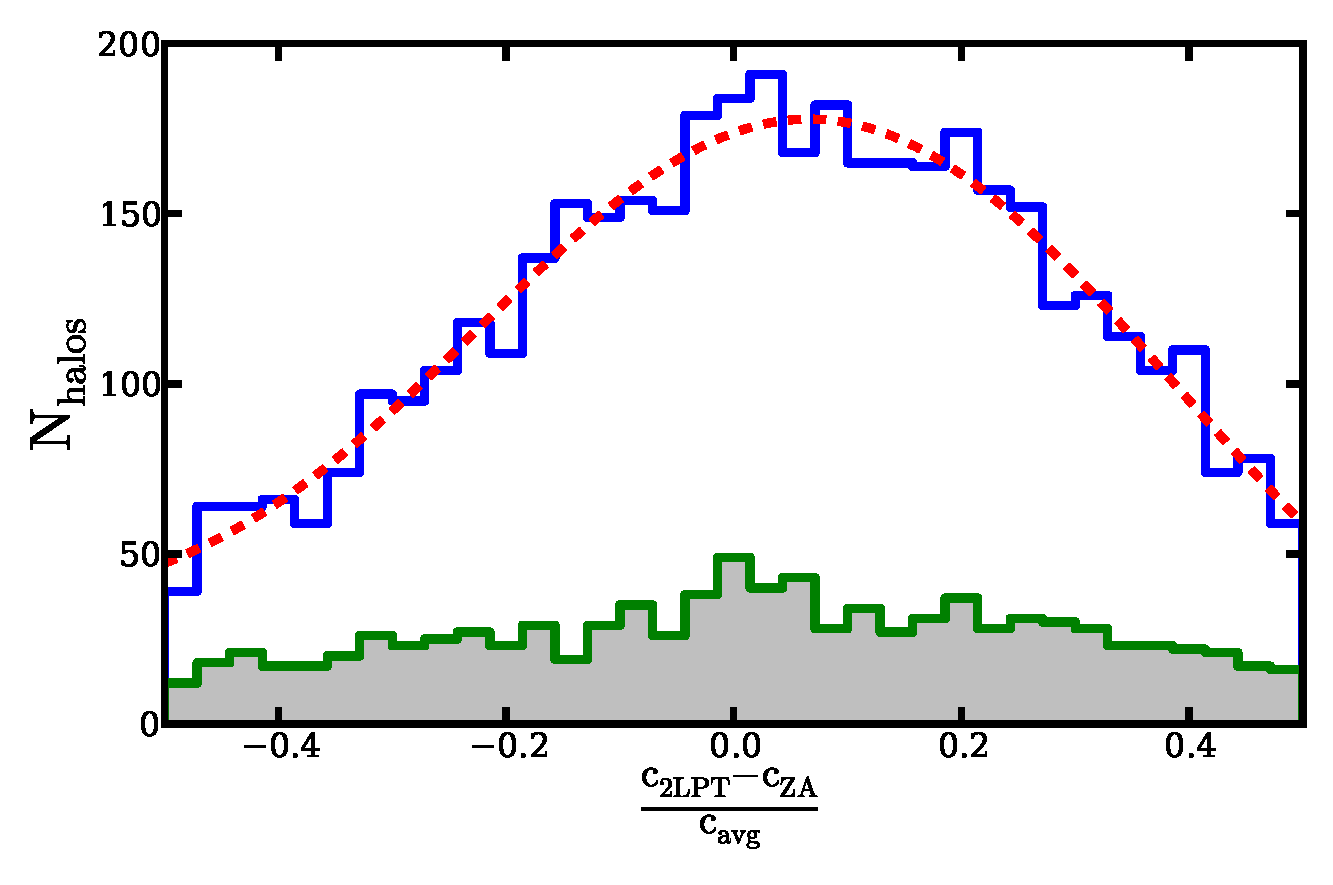
\includegraphics[width=0.48\linewidth]{diff-hist_c_snap040_(0.0-1.0).eps}
	\end{subfigure}
	\\
	\begin{subfigure}{}
		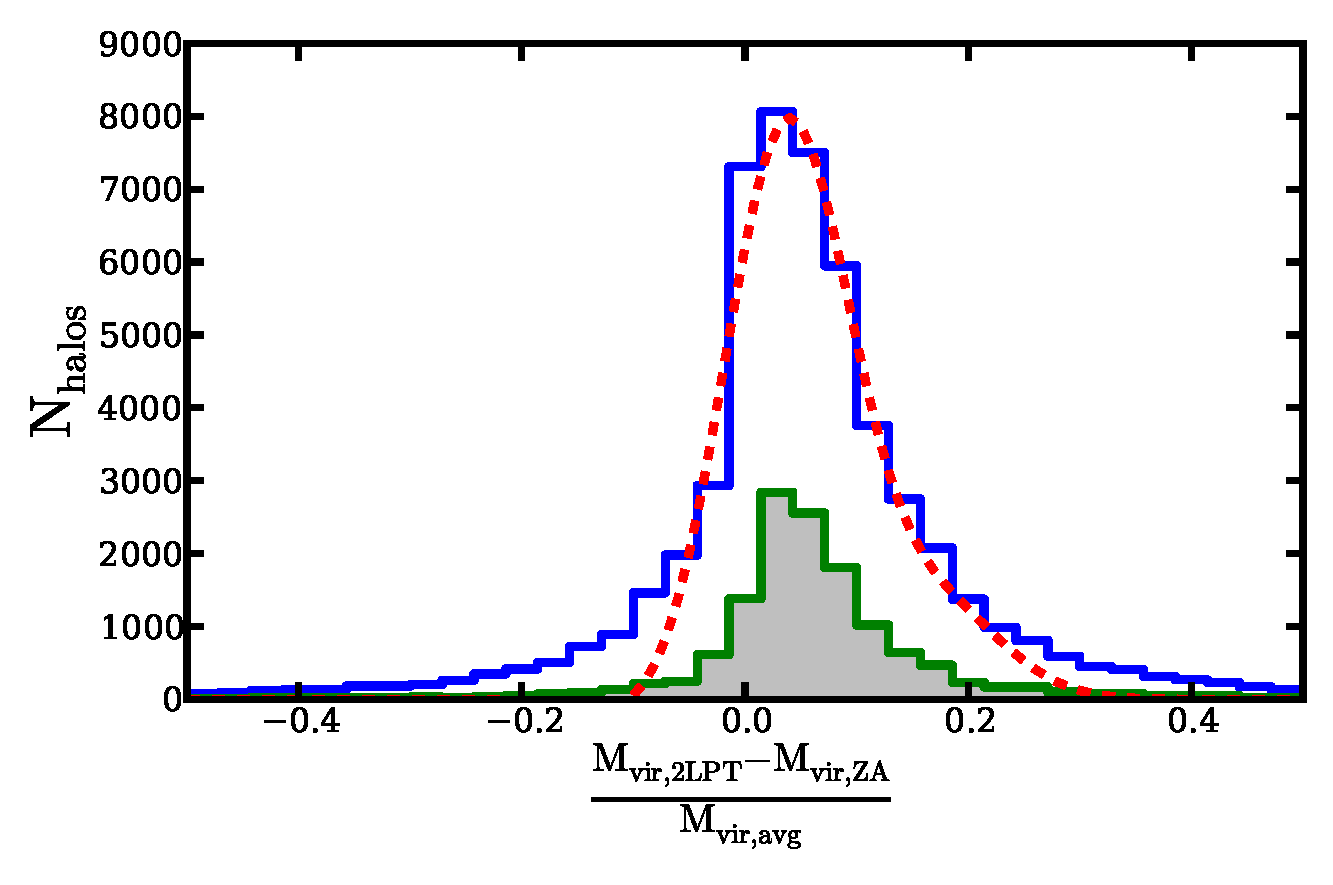
\includegraphics[width=0.48\linewidth]{diff-hist_Mvir_snap050_(0.0-1.0).eps}
	\end{subfigure}
	~
	\begin{subfigure}{}
		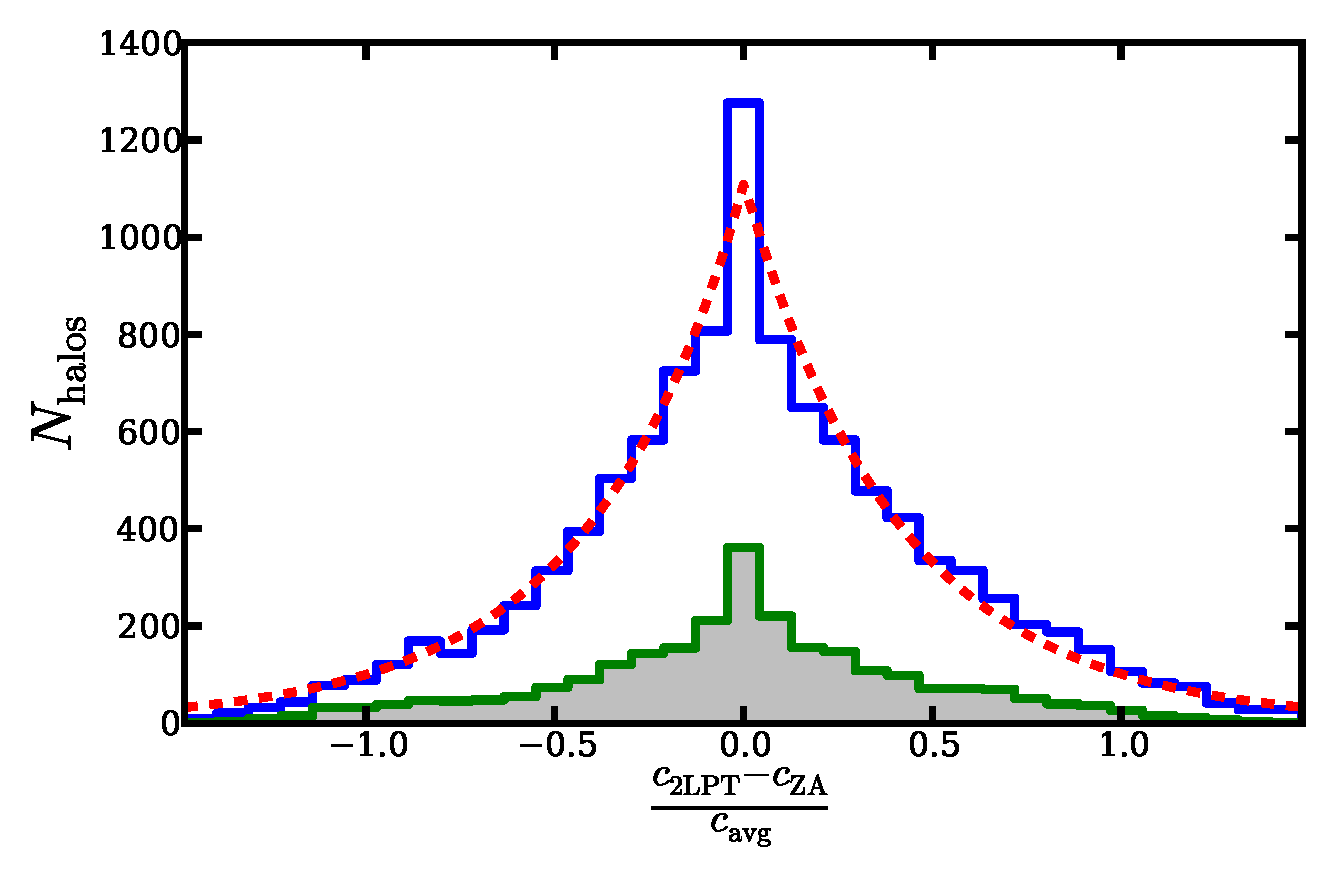
\includegraphics[width=0.48\linewidth]{diff-hist_c_snap050_(0.0-1.0).eps}
	\end{subfigure}
	\\
	\begin{subfigure}{}
		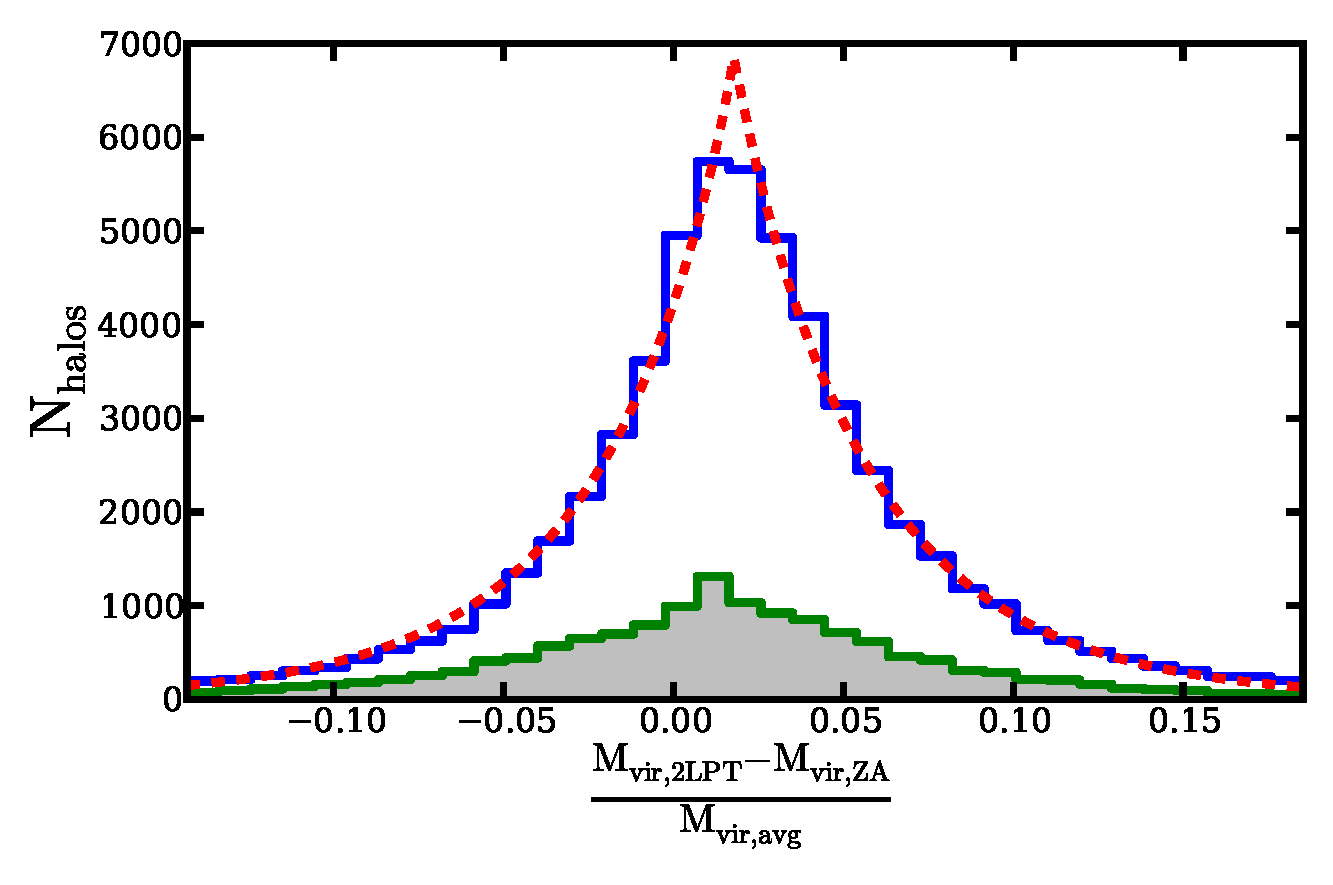
\includegraphics[width=0.48\linewidth]{diff-hist_Mvir_snap061_(0.0-1.0).eps}
	\end{subfigure}
	~
	\begin{subfigure}{}
		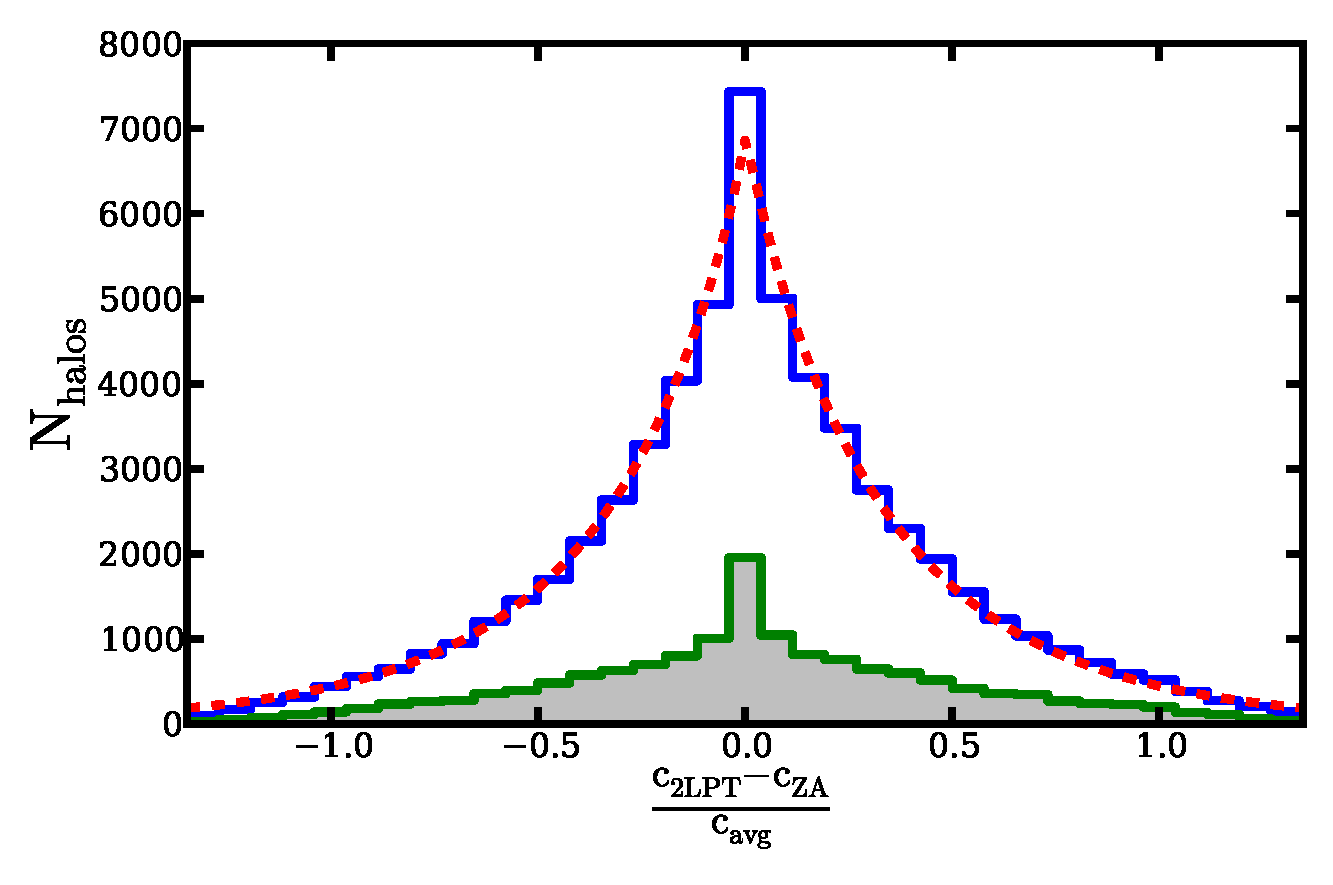
\includegraphics[width=0.48\linewidth]{diff-hist_c_snap061_(0.0-1.0).eps}
	\end{subfigure}
	\caption[Histograms of $\Delta M_{\mathrm{vir}}$ and $\Delta c$]{\footnotesize Histograms of $\Delta M_{\mathrm{vir}}$ (\textit{left column}) and $\Delta c$ (\textit{right column}) for snapshots at $z = 14.7$, $z = 10.3$, and $z = 6.0$ (\textit{top, middle, and bottom panels, respectively}).  The small gray-filled histograms count only the top 25\% most massive halos.  The main histograms are fit with a generalized normal distribution with parameters for mean, scale, and shape, overplotted as the red dashed line (see Equation~\ref{eq:generalized_normal}).  The distributions for $\Delta M_{\mathrm{vir}}$ have positive means and heavier \lpt\ halos, with the most pronounced difference at high redshift.  The distributions shown here have means of $(8.4 \pm 1.8) \times 10^{-2}$, $(4.87 \pm 0.87) \times 10^{-2}$, and $(1.79 \pm 0.31) \times 10^{-2}$, respectively.  The skew of the distribution is also the most positive at high redshift, and shifts toward symmetry by $z = 6$.  The $\Delta c$ distributions remain symmetric about zero and have negligible skew.  The means are consistent with zero, at $(2.6 \pm 2.7) \times 10^{-2}$, $(0.2 \pm 2.6) \times 10^{-2}$, and $(0.3 \pm 1.1) \times 10^{-2}$, respectively.  Both distributions have excess kurtosis consistently larger than that of a standard Gaussian distribution, with a sharp peak and heavy tails.}
	\label{fig:diff-hist}
\end{figure*}

For the halo population as a whole, we consider distributions of halo virial mass $M_{\mathrm{vir}}$ and concentration $c$.  We plot histograms of $\Delta M_{\mathrm{vir}}$ and $\Delta c$ in the left and right columns, respectively, of Figure~\ref{fig:diff-hist} for three representative timesteps at redshifts of $z = 14.7$, $z = 10.3$, and $z = 6.0$.  For each panel, the blue histogram features the entire halo sample, and the smaller gray-filled green histogram displays only the top 25\% most massive halos, ordered by \lpt\ mass.  Fits to the primary histograms are overplotted as red dashed curves.

Throughout the simulation, we find a tendency for \lpt\ halos to be more massive.  At $z = 15$, the mean of the $\Delta M_{\mathrm{vir}}$ distribution is $(9.3 \pm 1.2) \times 10^{-2}$.  The mean is consistently positive (heavier \lpt\ halos) and is most displaced from zero at high redshift.  The peak of the distribution gradually moves closer to zero as we progress in redshift.  We find the least difference between paired halos for the final snapshot at $z = 6$, with $\mu_{\Delta M_{\mathrm{vir}}} = (1.79 \pm 0.31) \times 10^{-2}$.

The higher-order moments of the $\Delta M_{\mathrm{vir}}$ distribution are of interest as well, as we find significant deviation from a Gaussian distribution.  As we use the symmetrical generalized normal distribution as our fit function, the skewness of the data is unable to be measured from the fit itself.  However, a qualitative deviation from symmetry can be readily observed.  By $z = 6$, we end up with a rather symmetrical distribution, with both sides of the histogram equally well described by our fit.  However, at higher redshift, we note a marked increase in skewness and deviation from this symmetry.  As redshift increases, we observe an increasing difference between the fit curve and the bins to the left of the histogram peak.

We find the distributions to be much closer to a Laplace distribution than a Gaussian, with shape parameter consistently sitting at or very close to $\beta = 1$.  Compared to a Gaussian distribution, the larger excess kurtosis implies a narrower central peak and heavier outlying tails.  Our fit constrains $\beta \geq 1$, so the kurtosis of the data itself could potentially be higher than the fit implies.

We find no no overall preference for more concentrated \lpt\ or \za\ halos.  In contrast to the $\Delta M_{\mathrm{vir}}$ histograms , $\Delta c$ shows very little deviation from symmetry about zero.  Throughout the simulation, we find the distributions to have a mean close to zero and negligible skew.  The widths of the distributions are much wider than those for $\Delta M_{\mathrm{vir}}$, with an order of magnitude difference by $z = 6$.  As with mass, concentration histograms are sharply peaked with heavy tails, implying a tendency for halo pairs to move towards the extremes of either very similar or very discrepant concentrations.




%~~~~~~~~~~~~~~~~~~~~~~~~~~~~~~~~~~~~~~~~~~~~~~~~~~~~~~~~~~~~~~~~~~~~~~~~~~~~~~~
\subsection{Trends with redshift}
%~~~~~~~~~~~~~~~~~~~~~~~~~~~~~~~~~~~~~~~~~~~~~~~~~~~~~~~~~~~~~~~~~~~~~~~~~~~~~~~


\begin{figure*}[t]
	\centering
	\begin{subfigure}{}
		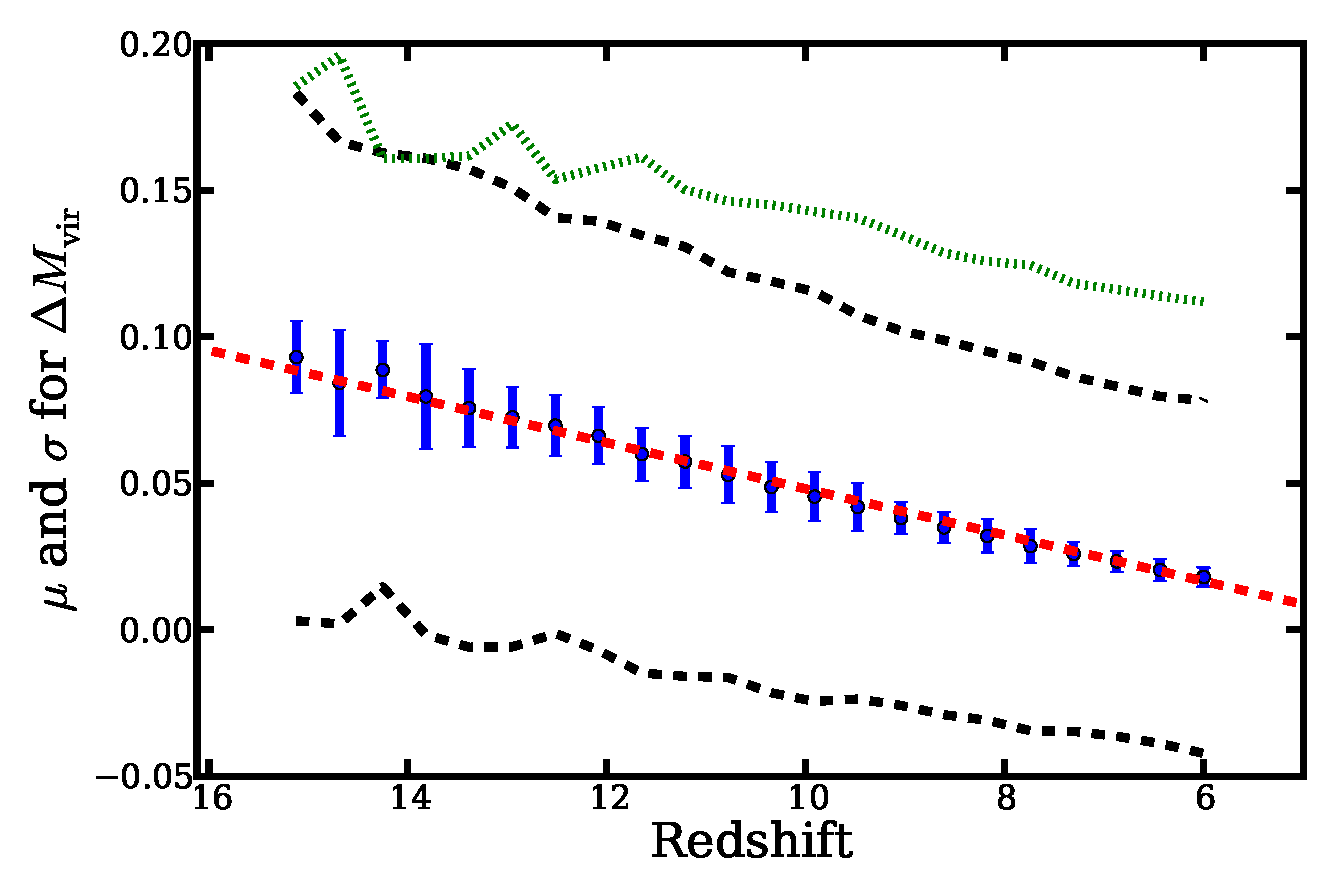
\includegraphics[width=0.48\linewidth]{mean_stdev_Mvir.eps}
	\end{subfigure}
	~
	\begin{subfigure}{}
		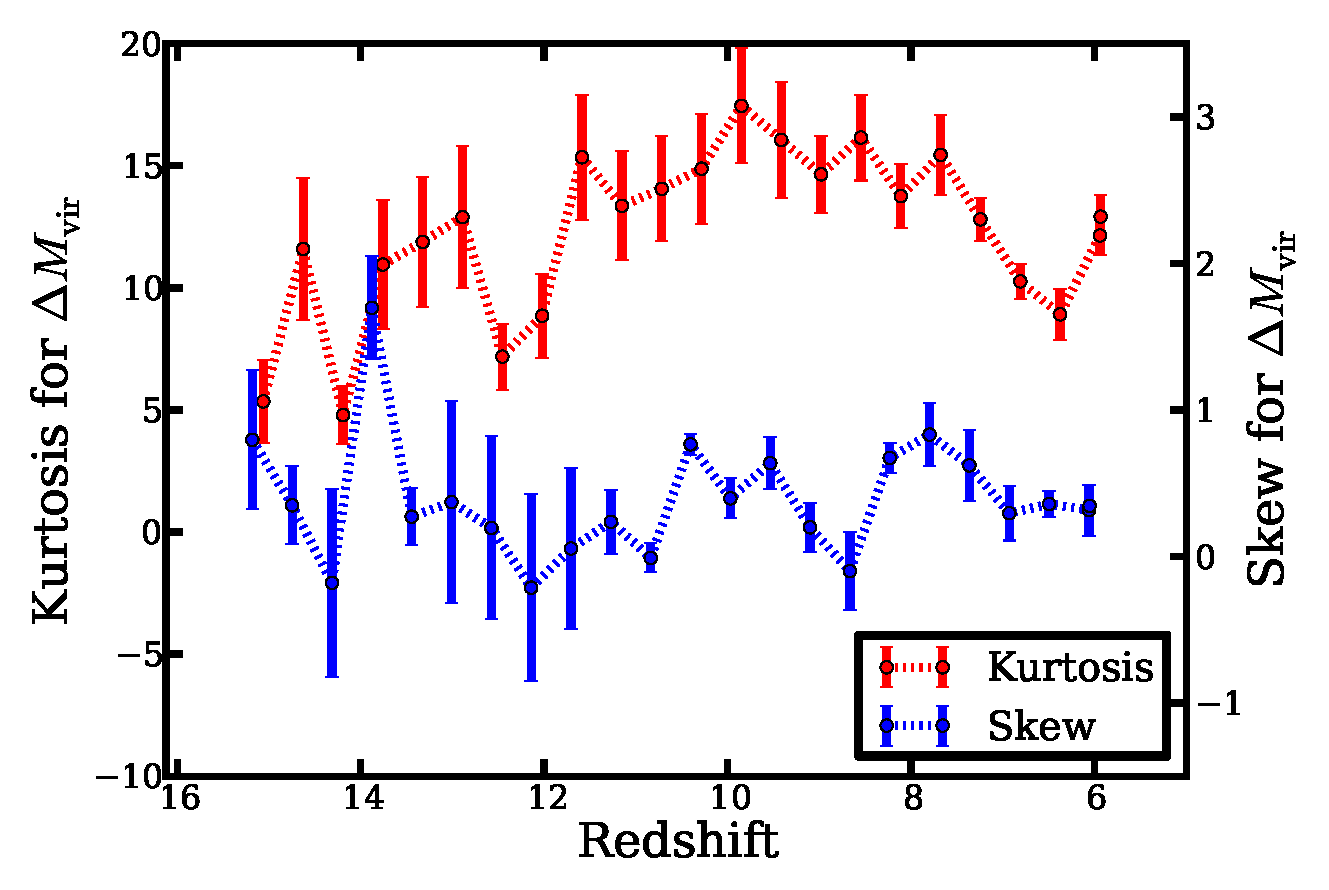
\includegraphics[width=0.48\linewidth]{skew_kurtosis_Mvir.eps}
	\end{subfigure}
	\\
	\begin{subfigure}{}
		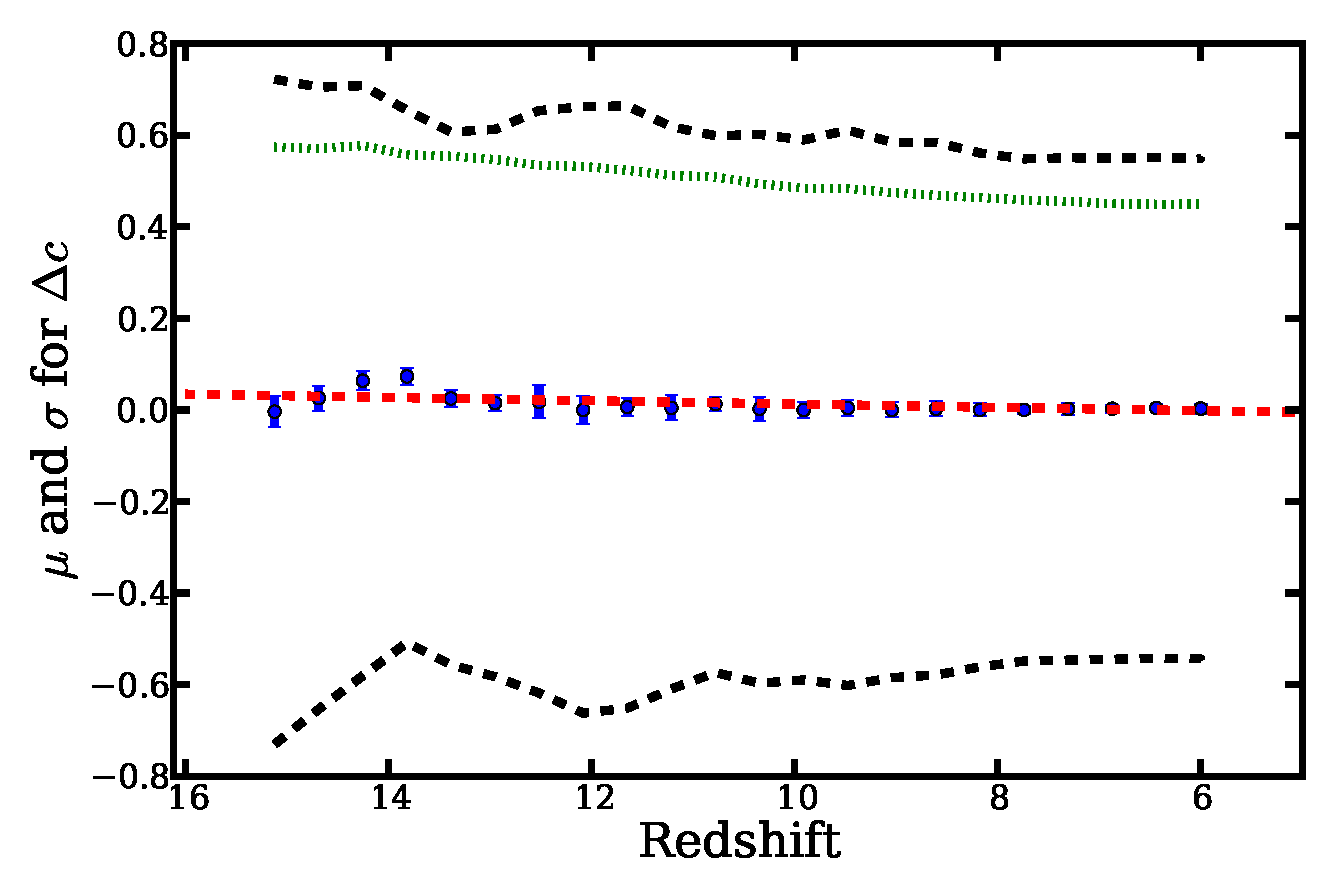
\includegraphics[width=0.48\linewidth]{mean_stdev_c_rockstar.eps}
	\end{subfigure}
	~
	\begin{subfigure}{}
		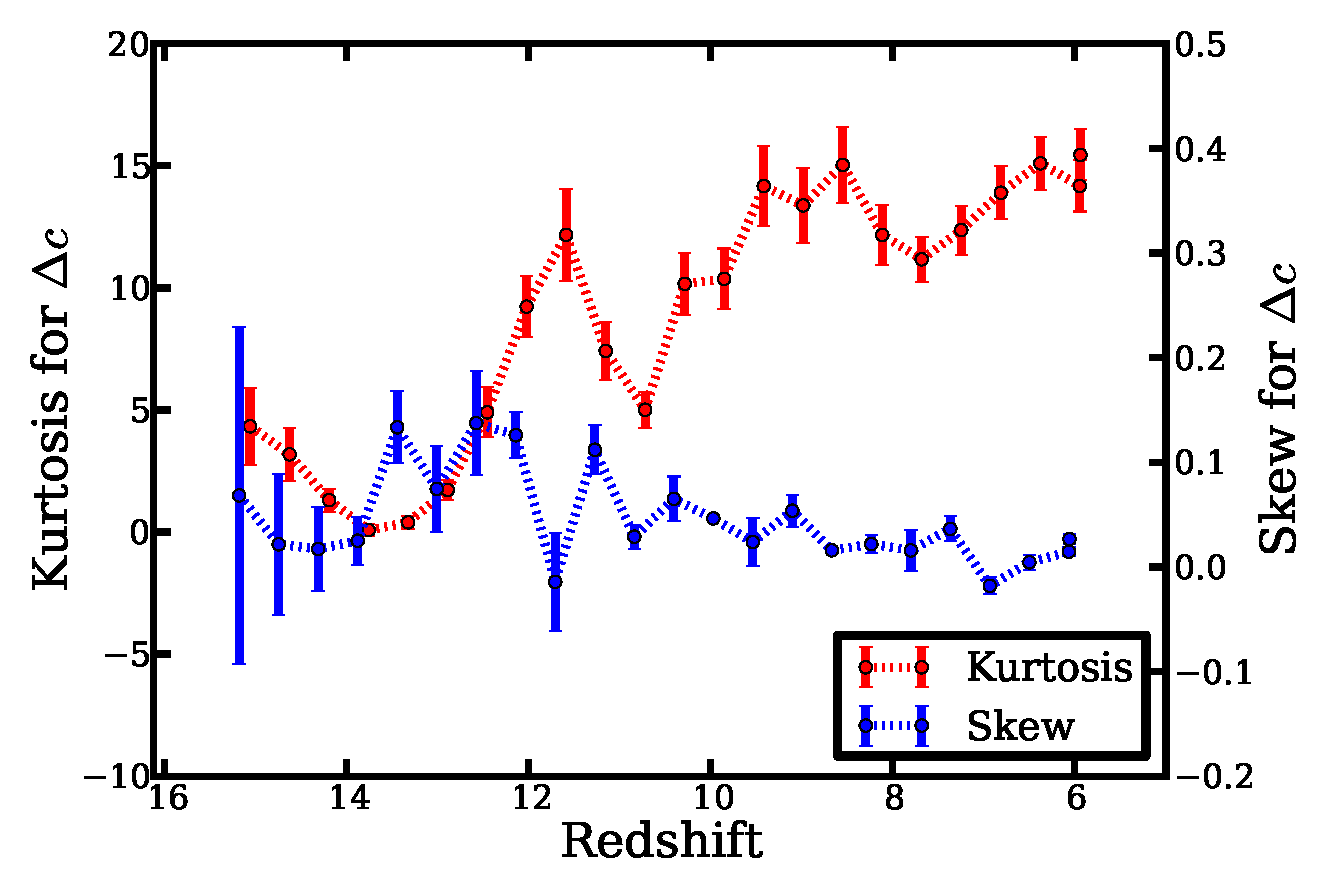
\includegraphics[width=0.48\linewidth]{skew_kurtosis_c_rockstar.eps}
	\end{subfigure}
	\caption[Statistics as functions of redshift for generalized normal fits]{\footnotesize Mean, standard deviation, and RMS (\textit{left column}) and skew and excess kurtosis (\textit{right column}) as functions of redshift for $\Delta M_{\mathrm{vir}}$ (\textit{top row}) and $\Delta c$ (\textit{bottom row}).  In the left column, $\mu$ is plotted as blue points, and $\mu \pm \sigma$ is plotted as the black dashed line, and RMS values are plotted as a green dotted line.  The red dashed line is a linear fit to the mean.  We find a significant trend for $\mu$ for $\Delta M_{\mathrm{vir}}$ to be more positive at higher redshift and gradually shift toward zero as the simulation progresses, with a fit function of $\mu_{\Delta M_{\mathrm{vir}}} = (7.88 \pm 0.17) \times 10^{-3} z - (3.07 \pm 0.14) \times 10^{-2}$.  The mean for $\Delta c$, however, remains at or very near zero for most of the simulation and is fit by $\mu_{\Delta c} = (3.62 \pm 0.95) \times 10^{-3} z - (2.34 \pm 0.84) \times 10^{-2}$.  The $\Delta M_{\mathrm{vir}}$ and $\Delta c$ distributions narrow over time, with a slight decrease in $\sigma$.  In the right column, we plot skew (blue line) and excess kurtosis (red line).  Skew is positive for much of the simulation for $\Delta M_{\mathrm{vir}}$, but is much smaller for $\Delta c$.  Kurtosis is large (much more peaked than Gaussian) for both $\Delta M_{\mathrm{vir}}$ and $\Delta c$ throughout much of the simulation, and especially at later redshift.}
	\label{fig:fit_trends}
\end{figure*}

In Figure~\ref{fig:fit_trends}, we more quantitatively assess the evolution of our various trends hinted at in Figure~\ref{fig:diff-hist}.  Here, we plot the mean, root mean square (RMS), standard deviation, skew, and kurtosis for $\Delta M_{\mathrm{vir}}$ and $\Delta c$ as functions of redshift.  Uncertainty in the mean is estimated directly by the least squares fitting routine.

The mean for $\Delta M_{\mathrm{vir}}$ is positive and highest at high redshift, trending toward zero by the end of the simulation.  Distributions for $\Delta c$ retain means close to and consistent with zero.  Standard deviation decreases slightly for both $\Delta M_{\mathrm{vir}}$ and $\Delta c$.  From $z = 15$ to $z = 6$, standard deviation falls from $(9.0 \pm 1.5) \times 10^{-2}$ to $(6.08 \pm 0.31) \times 10^{-2}$ for $\Delta M_{\mathrm{vir}}$ and from $0.73 \pm 0.11$ to $0.551 \pm 0.026$ for $\Delta c$.

\begin{table}[t]
	\centering
	\caption{Coefficients for linear least squares fits from Figure~\ref{fig:fit_trends}.}
	\begin{tabular}{ l  r  r }
		\toprule
		& \multicolumn{1}{c}{$\Delta M_{\mathrm{vir}}$} & \multicolumn{1}{c}{$\Delta c$} \\
		\cmidrule(l){2-3}
		A &  $(7.88 \pm 0.17) \times 10^{-3}$ &  $(3.62 \pm 0.95) \times 10^{-3}$ \\
		B & $(-3.07 \pm 0.14) \times 10^{-2}$ & $(-2.34 \pm 0.84) \times 10^{-2}$ \\
		\bottomrule
	\end{tabular}
	\label{tab:coeffs}
\end{table}

We find least square linear fits for both mean $\Delta M_{\mathrm{vir}}$ vs $z$ and mean $\Delta c$ vs $z$.  Coefficients for slope $A$ and y-intercept $B$ for the fit equation $\mu = A z + B$ are given in Table~\ref{tab:coeffs} for both cases.  We find a significant trend for $\Delta M_{\mathrm{vir}}$, with a slope $\sim 46 \sigma$ from zero.  Conversely, the slope for $\Delta c$ is much smaller and, considering the larger spread of the underlying distributions, can be considered negligible.  For $\Delta M_{\mathrm{vir}}$, the y-intercept coefficient $B$ likely has little meaning in terms of the actual behavior at $z = 0$, as we expect the trend to level out at later redshift.

We do note, however, that the mean can be deceiving as an indicator of total difference between halo populations, especially when it is close to zero as with concentration.  It should be noted that while the mean can indicate a lack of average difference between the whole sample of \lpt\ and \za\ halos, there can still be very large discrepancies between many individually paired halos.  We visualize this by plotting the RMS of $\Delta M_{\mathrm{vir}}$ and $\Delta c$, which is plotted as a green dotted line.  Unlike the mean, standard deviation,and kurtosis, which are measured from fits to the histograms, RMS is measured directly from the data and is not dependent on fitting.  The large RMS values are indicative of how much overall difference can arise between \lpt\ and \za\ halos, even though the differences may average to zero when considering the entire population.  The RMS for both $\Delta M_{\mathrm{vir}}$ and $\Delta c$ starts highest at high redshift---$0.19$ for $\Delta M_{\mathrm{vir}}$ and $0.57$ for $\Delta c$ at $z = 15$---and steadily decreases throughout the simulation, reaching minimums of $0.11$ for $\Delta M_{\mathrm{vir}}$ and $0.45$ for $\Delta c$ by $z = 6$.

Additionally, it is of interest to consider the percentage of halo pairs that are ``wrong'' at some given time, regardless of whether the quantity is higher in \lpt\ or \za.  For example, if we count halos outside a slit of $\epsilon = 10\%$ around $\Delta q = 0$, we find that by $z = 6$, 14.6\% of halo pairs still have substantially mismatched masses, and 74.3\% have mismatched concentrations.  It is evident that a substantial percentage of halo pairs can have markedly different growth histories, even when there is little or no offset in the ensemble halo population average.

Kurtosis is consistently large for both mass and concentration, with a slight increasing trend throughout the simulation for concentration.  It reaches maximum values of $17.5 \pm 2.4$ at redshift 10 for $\Delta M_{\mathrm{vir}}$ and $15.4 \pm 1.0$ at the end of the simulation at redshift 6 for $\Delta c$.  Skew is positive for much of the simulation for mass, but is much smaller for concentration.  We find average skews of $0.39 \pm 0.29$ for $\Delta M_{\mathrm{vir}}$ and $0.045 \pm 0.028$ for $\Delta c$.  These higher moment deviations from Gaussianity hint at the non-linear dynamics at play in halo formation.

The narrow peak and heavy tails of the distribution may indicate a fair amount of sensitivity to initial differences in halo properties, in that halo pairs that start out within a certain range of the mean are more likely move closer to the mean, while pairs that are initially discrepant will diverge even further in their characteristics.  This is indicative of the non-linear gravitational influence present during halo evolution, and is further supported by a kurtosis that increases with time.

The skew at high redshift for $\Delta M_{\mathrm{vir}}$ may give another hint at the non-linear halo formation process.  Runaway halo growth causes more massive halos to favor faster mass accretion and growth.  The positively skewed distributions show a picture of \lpt\ halo growth in which initial differences in mass are amplified the most readily in the earliest forming and most massive halos, again indicating the extra kick-start to halo growth provided by \lpt\ initialization.  While the slight decrease in skew with redshift may be counter-intuitive to this notion, it is likely that the large number of newly formed halos begin to mask the signal from the smaller number of large halos displaying this effect.




%~~~~~~~~~~~~~~~~~~~~~~~~~~~~~~~~~~~~~~~~~~~~~~~~~~~~~~~~~~~~~~~~~~~~~~~~~~~~~~~
\subsection{Trends with halo mass}
%~~~~~~~~~~~~~~~~~~~~~~~~~~~~~~~~~~~~~~~~~~~~~~~~~~~~~~~~~~~~~~~~~~~~~~~~~~~~~~~


\begin{figure*}[t]
	\centering
	\begin{subfigure}{}
		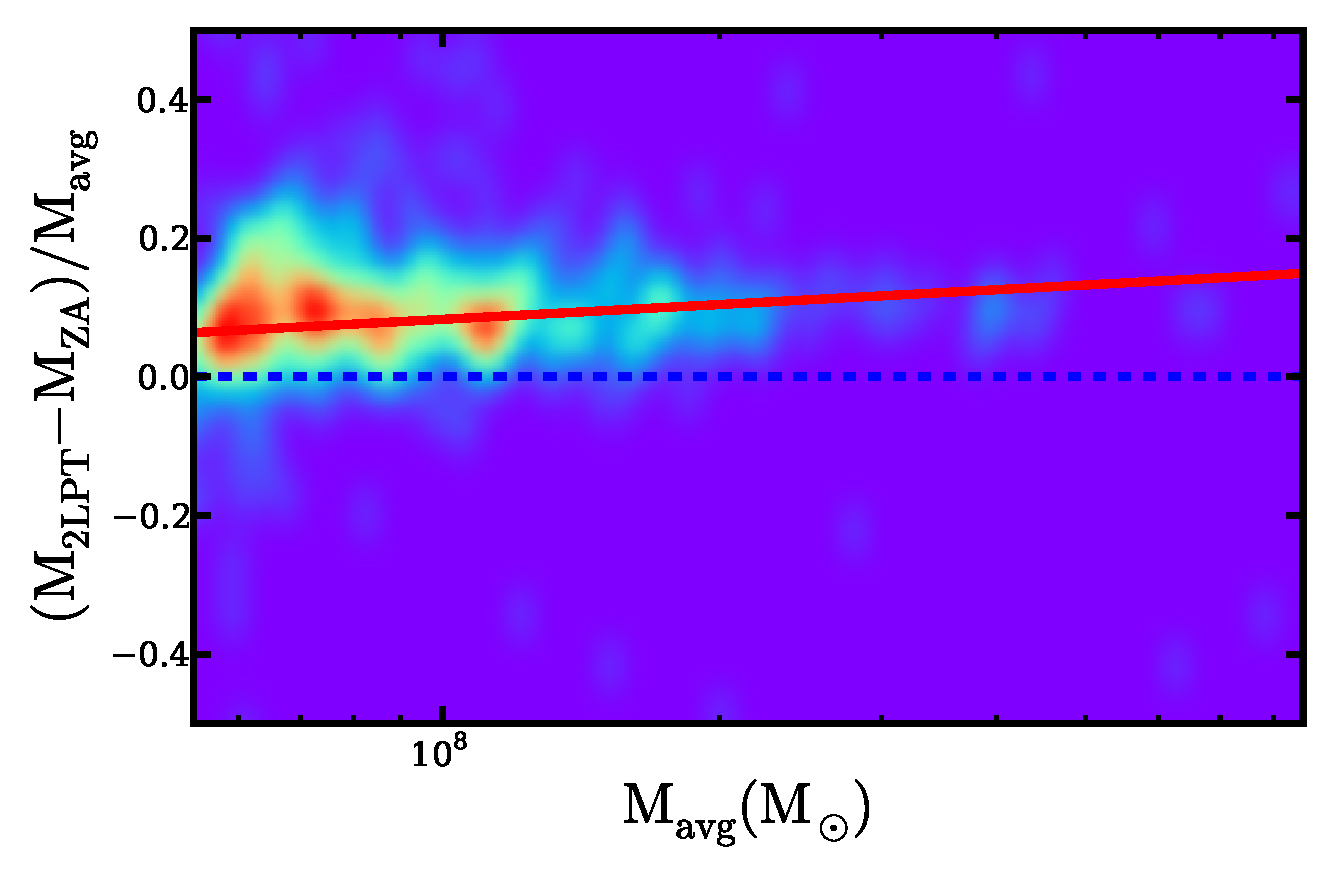
\includegraphics[width=0.48\linewidth]{dM-v-Mavg_snap040.eps}
	\end{subfigure}
	~
	\begin{subfigure}{}
		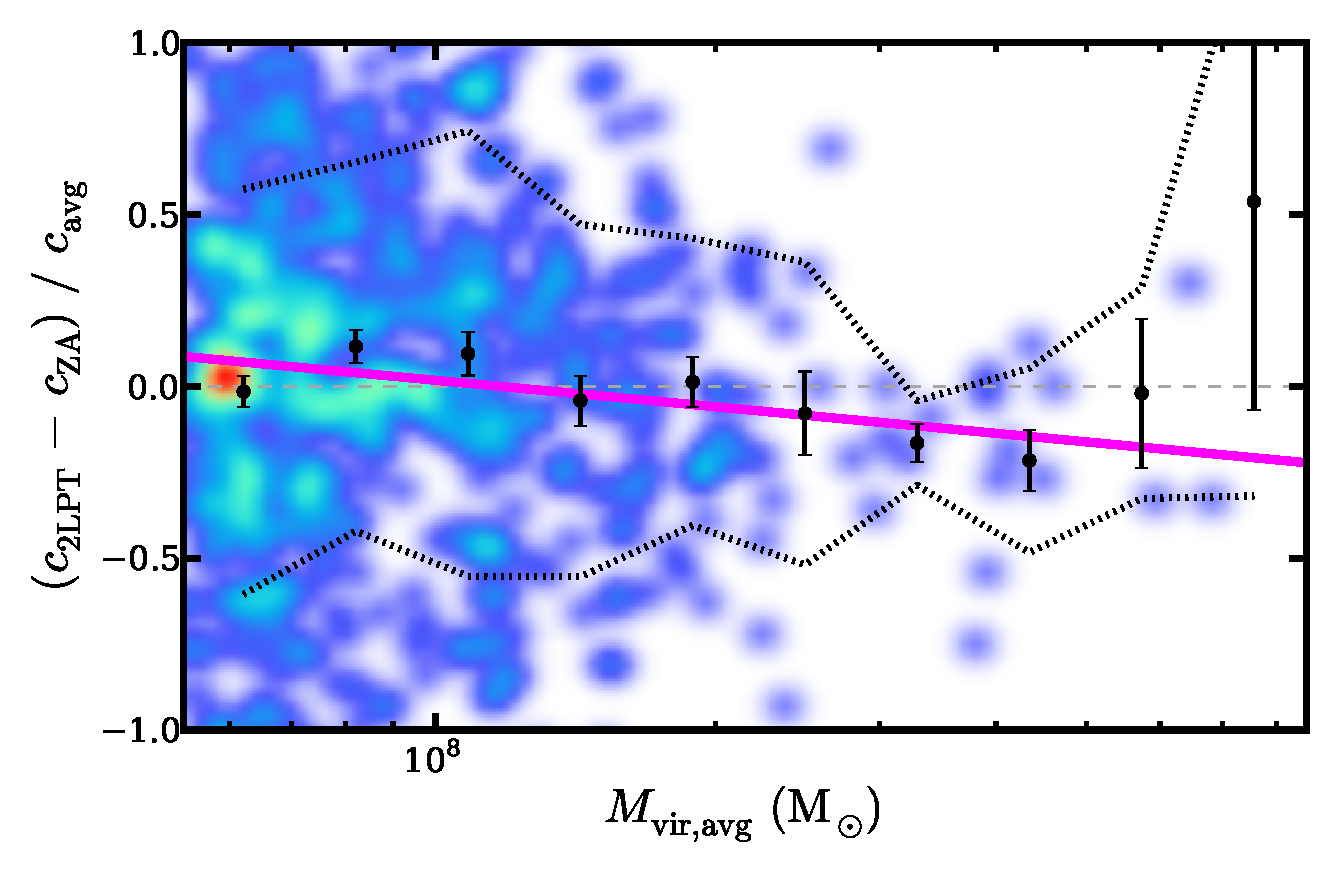
\includegraphics[width=0.48\linewidth]{dc-v-Mavg_snap040.eps}
	\end{subfigure}
	\\
	\begin{subfigure}{}
		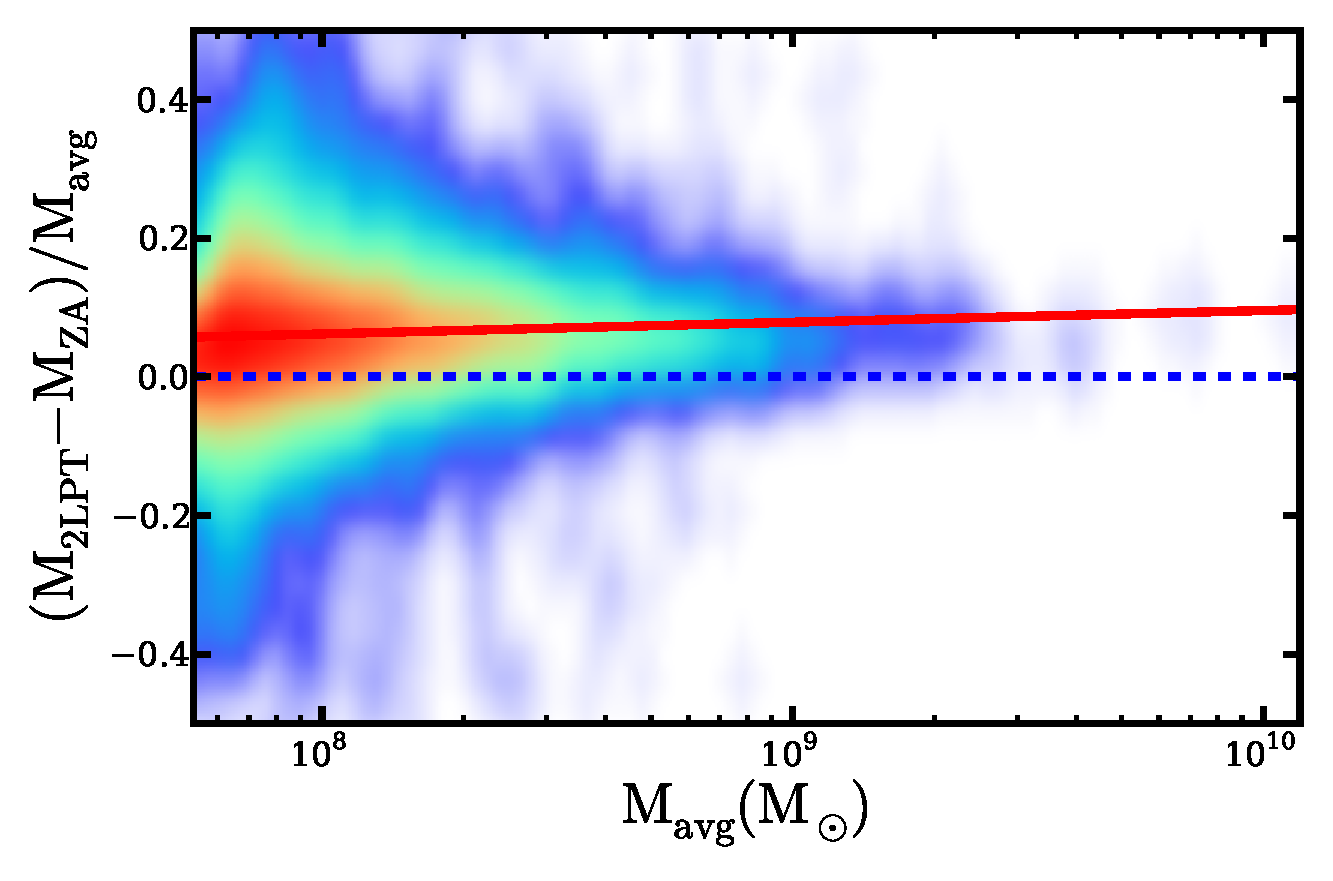
\includegraphics[width=0.48\linewidth]{dM-v-Mavg_snap050.eps}
	\end{subfigure}
	~
	\begin{subfigure}{}
		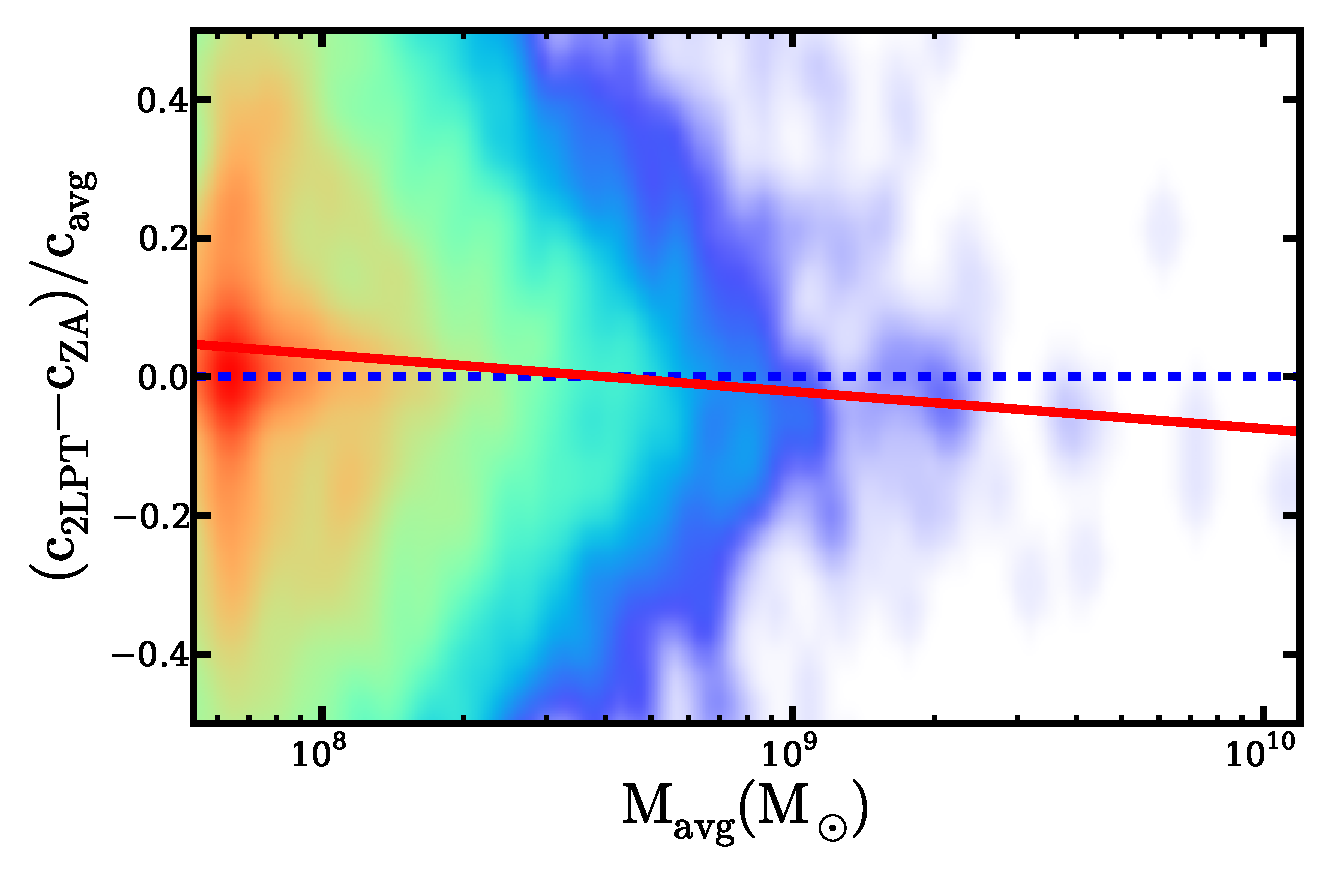
\includegraphics[width=0.48\linewidth]{dc-v-Mavg_snap050.eps}
	\end{subfigure}
	\\
	\begin{subfigure}{}
		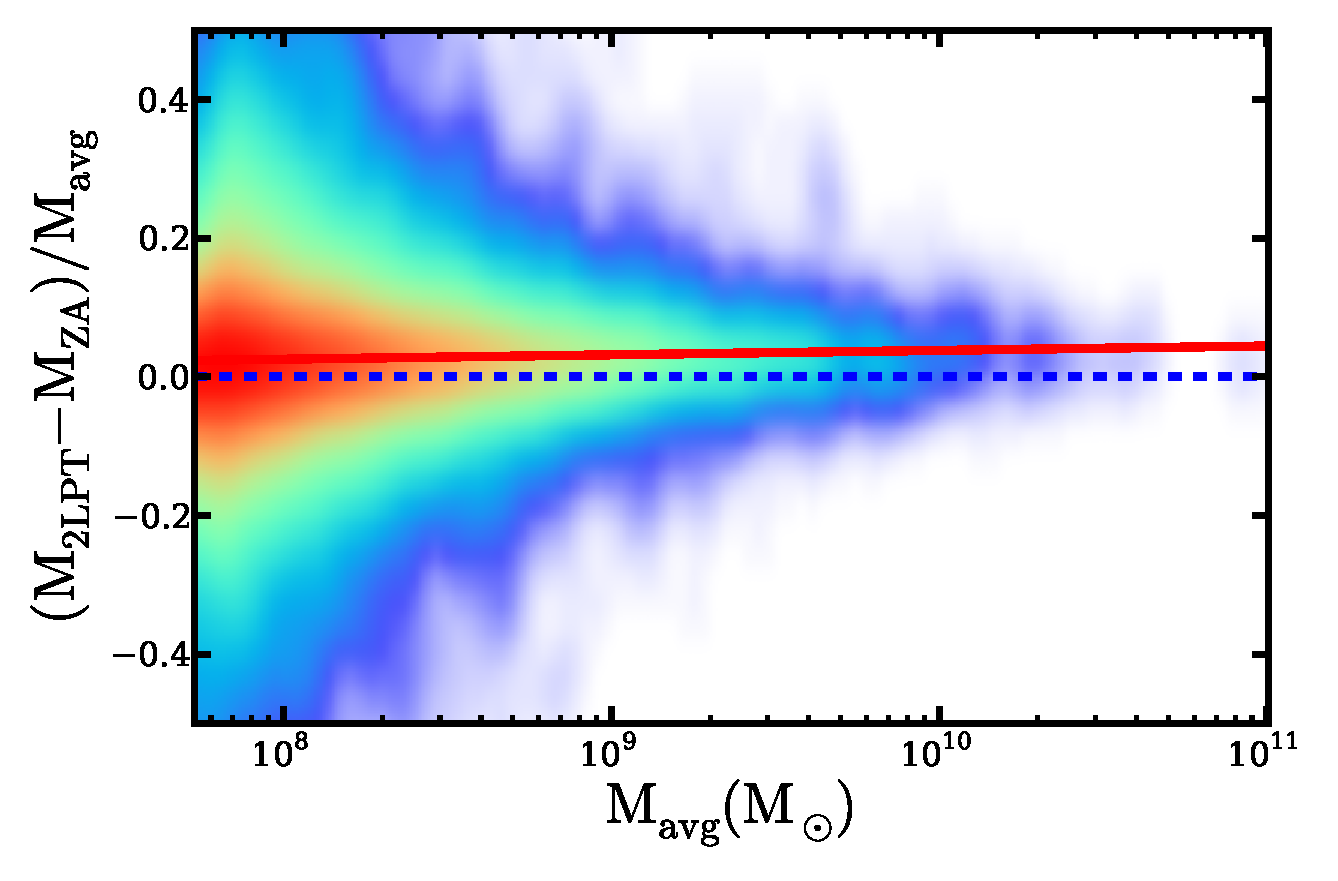
\includegraphics[width=0.48\linewidth]{dM-v-Mavg_snap061.eps}
	\end{subfigure}
	~
	\begin{subfigure}{}
		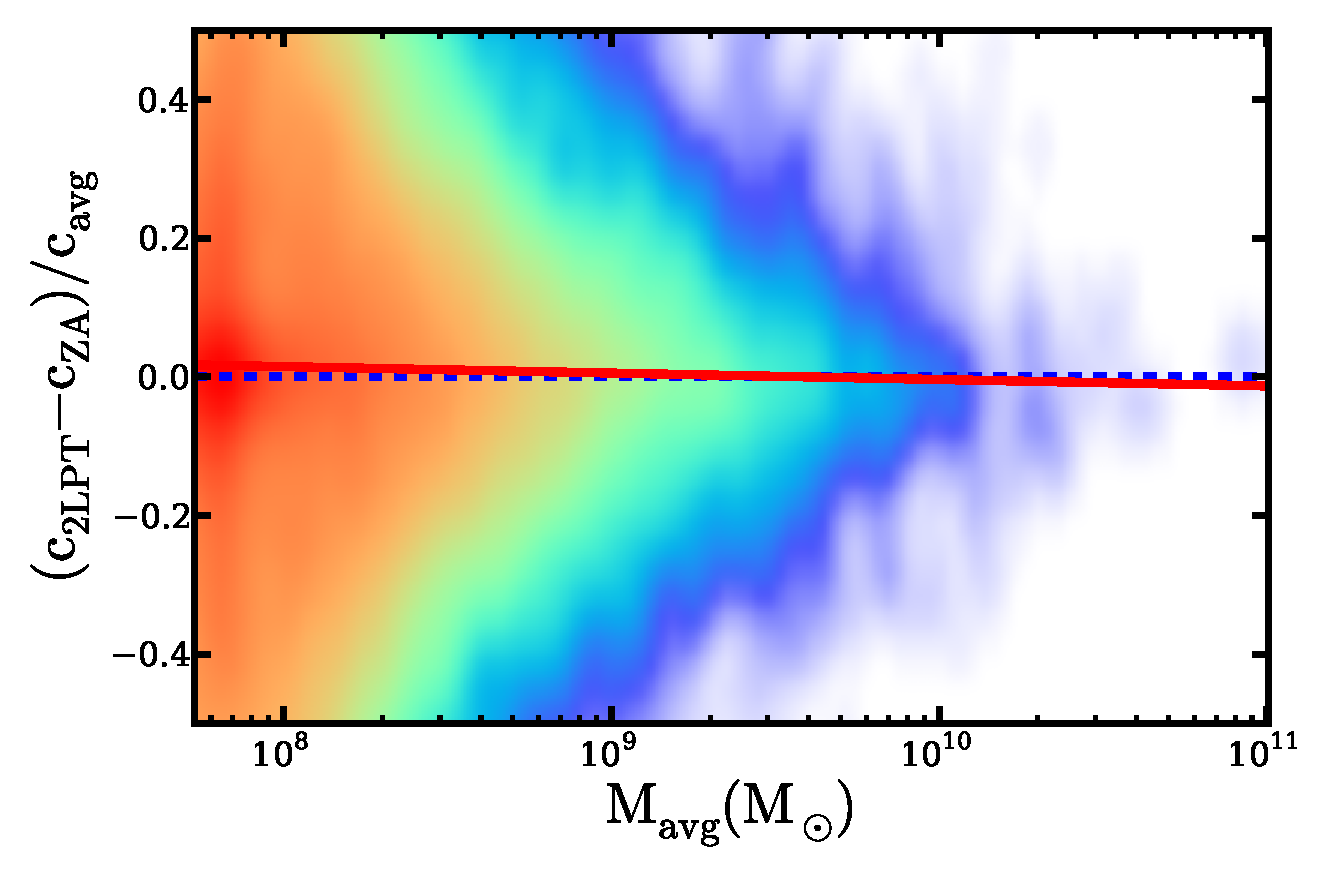
\includegraphics[width=0.48\linewidth]{dc-v-Mavg_snap061.eps}
	\end{subfigure}
	\caption[$\Delta M_{\mathrm{vir}}$ and $\Delta c$ as a function of $M_{\mathrm{vir,avg}}$]{\footnotesize $\Delta M_{\mathrm{vir}}$ (left column) and $\Delta c$ (right column) as functions of $M_{\mathrm{vir,avg}}$.  Halos are counted in 2-D rectangular bins and smoothed with a Gaussian kernel with a logarithmic color scale.  The red line is the least-squares best fit to the data.  The blue dashed line at zero is provided to guide the eye.  The three rows again correspond to snapshots at $z = 14.7$, $z = 10.3$, and $z = 6.0$.  We again see the overall offset for positive $\Delta M_{\mathrm{vir}}$ as before, and additionally find that more massive halo pairs are more likely to have even larger $\Delta M_{\mathrm{vir}}$, especially at high redshift.  Fit equations for the left column panels are $\Delta M_{\mathrm{vir}} = 5.6 \times 10^{-2} M_{\mathrm{vir,avg}} - 0.33$, $\Delta M_{\mathrm{vir}} = 1.7 \times 10^{-2} M_{\mathrm{vir,avg}} - 7.3 \times 10^{-2}$, and $\Delta M_{\mathrm{vir}} = 6.4 \times 10^{-3} M_{\mathrm{vir,avg}} - 2.5 \times 10^{-2}$, respectively.  Concentration show a small but opposite trend for more massive halos to be more concentrated in \za\ than in \lpt.  The right column panels have fit equations $\Delta c = -5.3 \times 10^{-2} M_{\mathrm{vir,avg}} + 0.46$, $\Delta c = -4.5 \times 10^{-2} M_{\mathrm{vir,avg}} + 0.46$, and $\Delta c = -9.3 \times 10^{-3} M_{\mathrm{vir,avg}} + 8.9 \times 10^{-2}$, respectively.}
	\label{fig:delta-v-Mavg}
\end{figure*}

We consider $\Delta M_{\mathrm{vir}}$ and $\Delta c$ as a function of average halo mass $M_{\mathrm{vir,avg}} = (M_{\mathrm{vir},\lpt} + M_{\mathrm{vir},\za}) / 2$ in Figure~\ref{fig:delta-v-Mavg}.  The data is binned on a 2-D grid with a logarithmic color map for three representative timesteps.  A linear fit to the data is overplotted in red, and a dotted blue line is provided at $\Delta M_{\mathrm{vir}} = 0$ and $\Delta c = 0$ to guide the eye.

We find that $\Delta M_{\mathrm{vir}}$ tends to increase with increasing $M_{\mathrm{vir,avg}}$, a trend that is, again, most pronounced at high redshift.  \lpt\ halos are consistently more massive than their \za\ counterparts, with the difference increasing with average halo mass.  While less massive halo pairs have a larger spread in the difference in \lpt\ and \za\ mass, more massive halo pairs are consistently heavier in \lpt\ than in \za.  At redshift 15, the least squares fit to the data produces the fit equation $\Delta M_{\mathrm{vir}} = 5.6 \times 10^{-2} M_{\mathrm{vir,avg}} - 0.33$.   The slope of the fit line trends towards zero as we progress in redshift, with little average mass dependence and a fit of $\Delta M_{\mathrm{vir}} = 6.4 \times 10^{-3} M_{\mathrm{vir,avg}} - 2.5 \times 10^{-2}$ by $z = 6$.

We find a small trend for more massive halo pairs to be more concentrated in \za, but this trend is weaker than for $\Delta M_{\mathrm{vir}}$.  The fit equations for $z = 15$ and $z = 6$ are $\Delta c = -5.3 \times 10^{-2} M_{\mathrm{vir,avg}} - 0.45$ and $\Delta c = -9.3 \times 10^{-3} M_{\mathrm{vir,avg}} - 8.9 \times 10^{-2}$, respectively.  The negative slope might be expected, as halo concentration is expected to decrease with increasing mass, at least at later redshift \citep{2007MNRAS.381.1450N}, and we find high mass halos to be more massive in \lpt\ than in \za.  However, the dependence of concentration on mass and redshift at high redshift is more complicated \citep{2011ApJ...740..102K, 2012MNRAS.423.3018P}.  The data have a larger variance than $\Delta M_{\mathrm{vir}}$, and fits have and overall shallower slope.  Mass dependence all but disappears by $z = 6$.  To reconcile these trends with the symmetrical concentration distributions of Figure~\ref{fig:diff-hist}, we note that the trends in mass may be hidden by integration across the entire mass range and still result in overall $\Delta c$ distributions symmetric about zero.




%~~~~~~~~~~~~~~~~~~~~~~~~~~~~~~~~~~~~~~~~~~~~~~~~~~~~~~~~~~~~~~~~~~~~~~~~~~~~~~~
\subsection{Alternate fractional difference distributions}
%~~~~~~~~~~~~~~~~~~~~~~~~~~~~~~~~~~~~~~~~~~~~~~~~~~~~~~~~~~~~~~~~~~~~~~~~~~~~~~~


\begin{figure*}[t]
	\centering
	\begin{subfigure}{}
		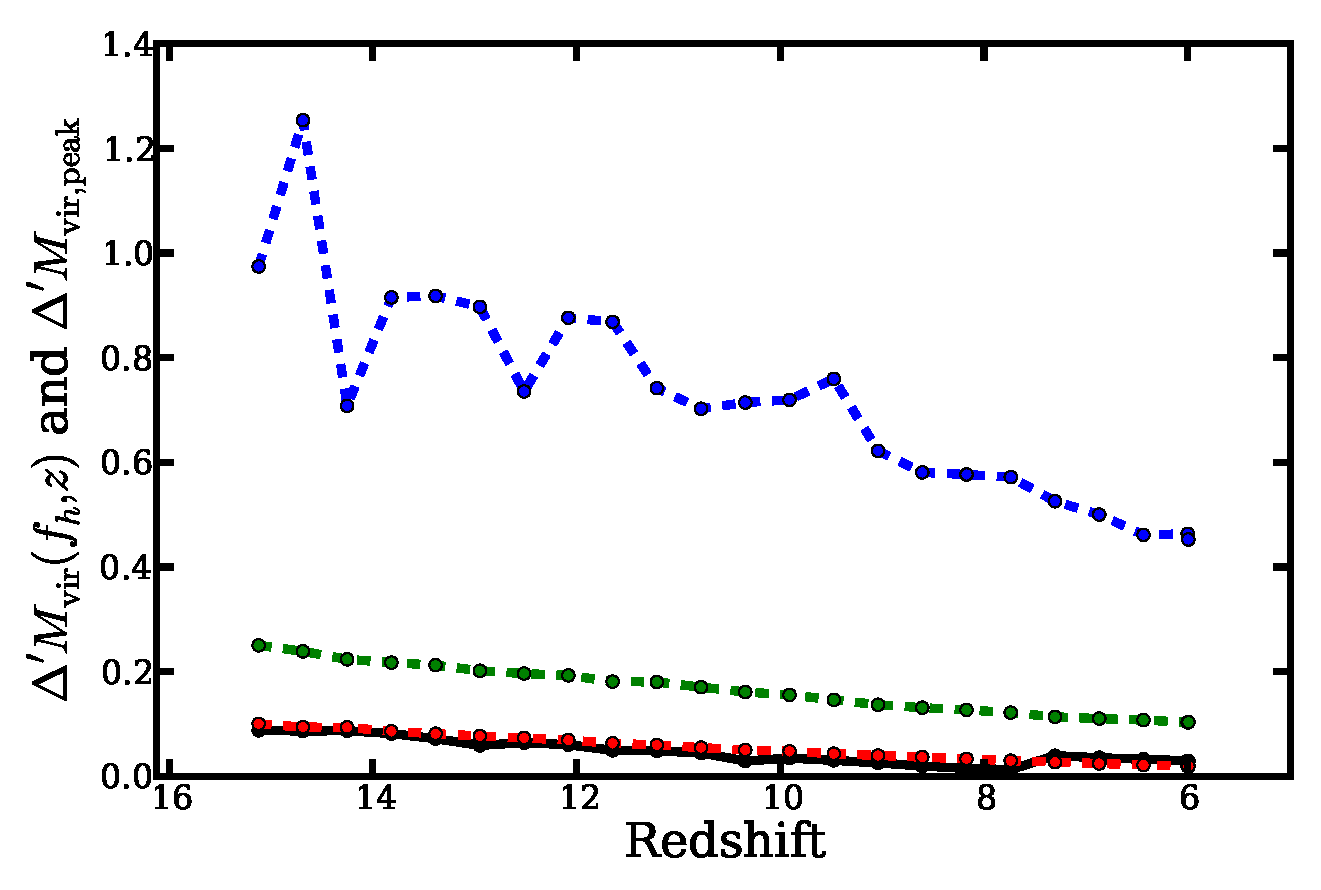
\includegraphics[width=0.48\linewidth]{percdiff_Mvir_xvals.eps}
	\end{subfigure}
	~
	\begin{subfigure}{}
		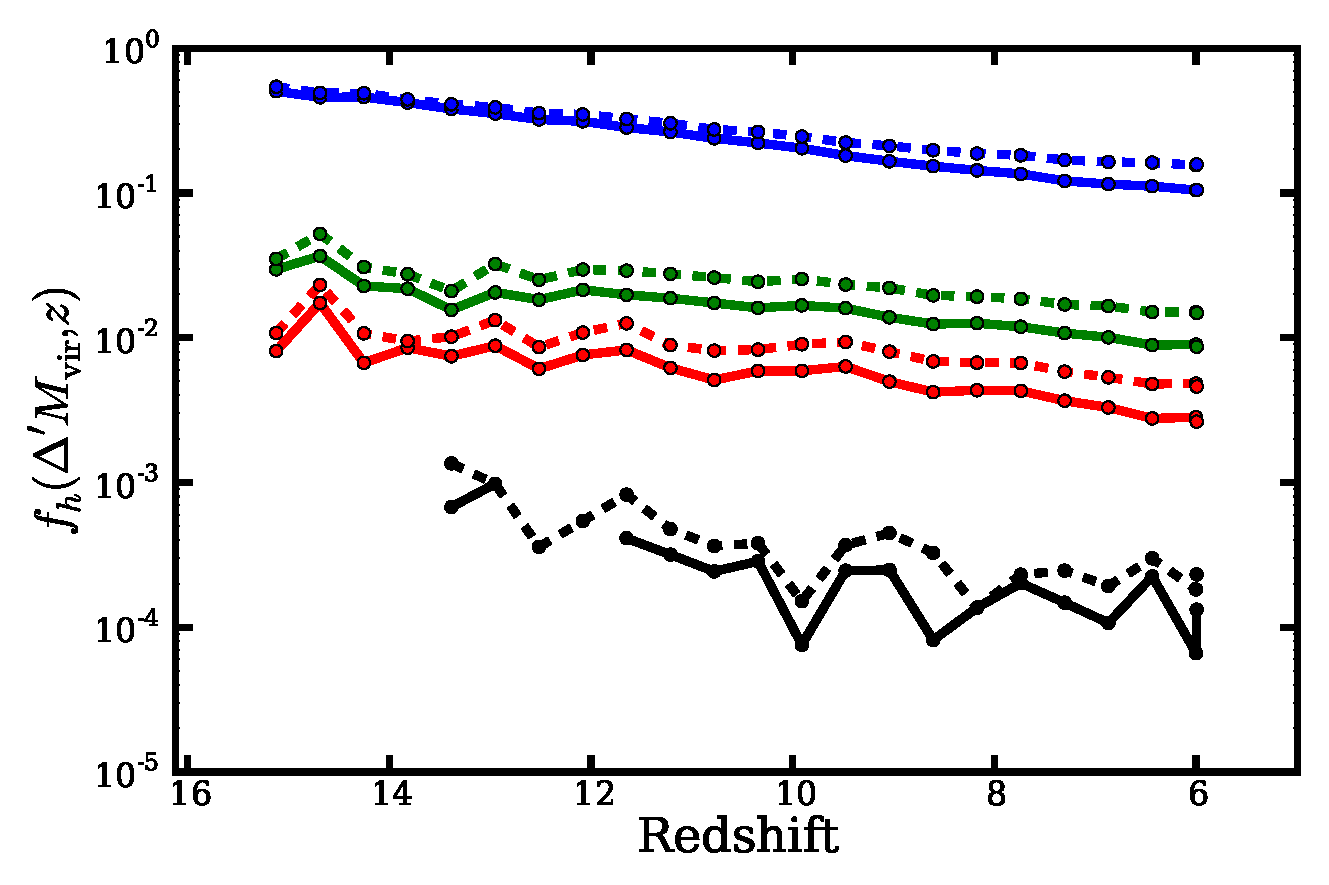
\includegraphics[width=0.48\linewidth]{percdiff_Mvir_sumfrac.eps}
	\end{subfigure}
	\\
	\begin{subfigure}{}
		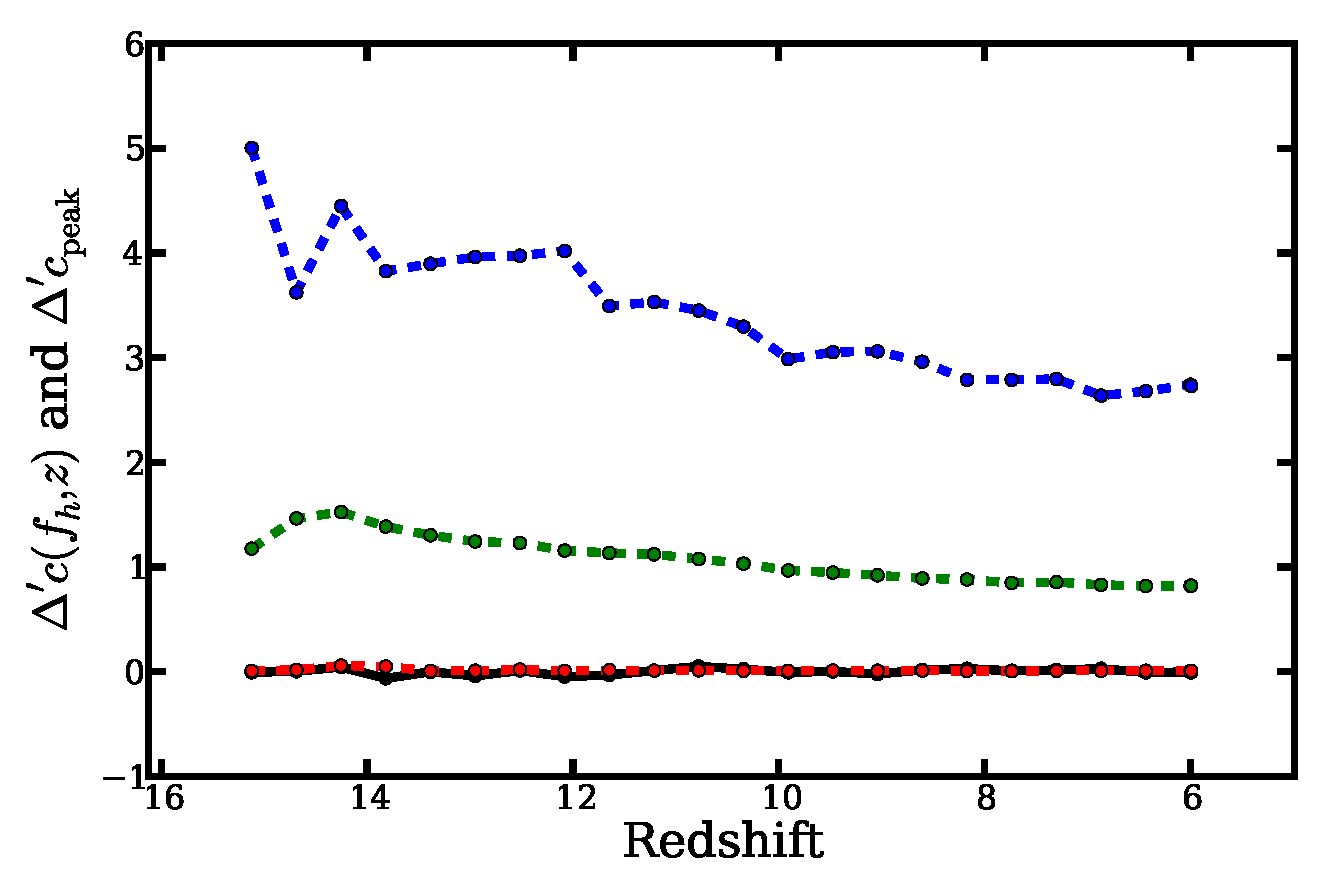
\includegraphics[width=0.48\linewidth]{percdiff_c_rockstar_xvals.eps}
	\end{subfigure}
	~
	\begin{subfigure}{}
		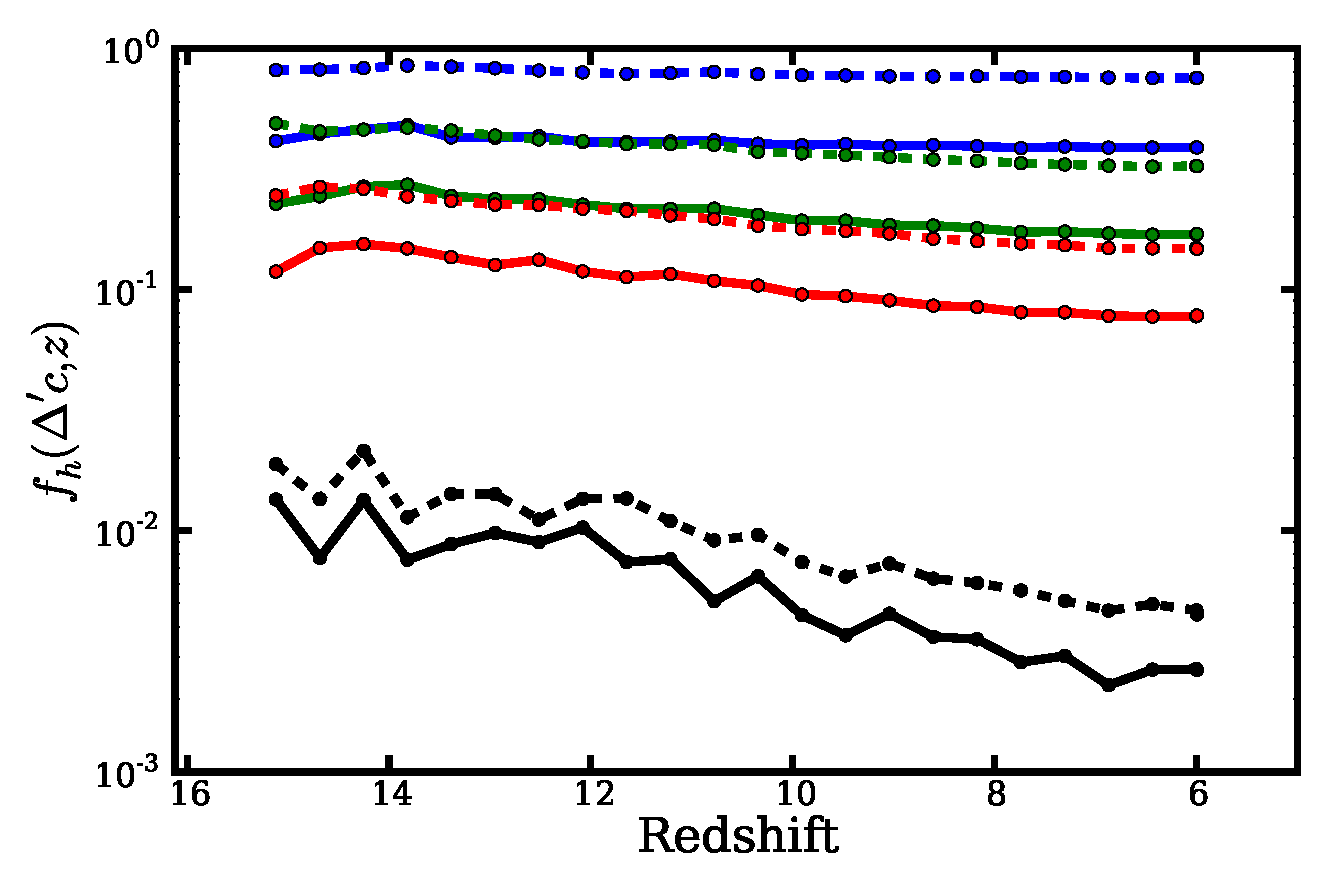
\includegraphics[width=0.48\linewidth]{percdiff_c_rockstar_sumfrac.eps}
	\end{subfigure}
	\caption[Fractional error distribution statistics as functions of redshift]{\footnotesize Fractional error distributions statistics for $\Delta' M_{\mathrm{vir}}$ (\textit{top row}) and $\Delta' c$ (\textit{bottom row}) as functions of redshift.  \textit{Left column}:  The $\Delta' q$ of the peak of the distribution (black line), and the $\Delta' q$ where 50\% (red dashed line), 10\% (green dashed line), and 1\% (blue dashed line) of the halos fall at or above $\Delta' q$.  As with distributions of $\Delta M_{\mathrm{vir}}$, $\Delta' M_{\mathrm{vir}}$ has the largest positive displacement at high redshift and steadily decreases throughout the simulation.  Additionally, $\Delta' c$ maintains a peak near zero and has a spread much larger than that of $\Delta' M_{\mathrm{vir}}$.  \textit{Right column}:  The fraction of halos with $\Delta' q$ greater than 0.10 (solid blue line), 0.50 (solid green line), 1.00 (solid red line), and 4.00 (solid black line).  The dashed lines additionally count halo pairs with $\Delta' q$ lower than the corresponding equivalent displacements of -0.09, -0.33, -0.50, and -0.80, respectively (see Equation~\ref{eq:equivalent_q_prime}).  We find that 50\% of \lpt\ halos are at least 10\% more massive than their \za\ companions at $z = 15$, reducing to 10\% by $z = 6$.  Halos in \lpt\ are at least twice as concentrated for 12\% of halos at $z = 15$ and 7.8\% of halos at $z = 6$.}
	\label{fig:frac_err_trends}
\end{figure*}

In Figure~\ref{fig:frac_err_trends}, we plot, as functions of redshift, statistics derived from the alternate fractional difference distributions $\Delta' M_{\mathrm{vir}}$ and $\Delta' c$ (see Equation~\ref{eq:delta_prime_q}).  In the left column, we plot the $\Delta' q$ of the peak of the distribution along with the $\Delta' q$ where various percentages of the halo pairs fall at or above $\Delta' q$.

As the $\Delta' q$ value of peak of the distribution is the location of the mode, it represents the most typical halo pair.  While concentration differences remain close to zero throughout the simulation, mass difference peak moves from a $\Delta' M_{\mathrm{vir}}$ of $8.7 \times 10^{-2}$ at $z = 15$ to $2.9 \times 10^{-2}$ at $z = 6$.  The 1\% of halo pairs with the largest excess \lpt\ mass are at least 1.97 times \za\ mass at $z = 15$ and 1.45 times \za\ mass at $z = 6$.  For concentration, the 1\% most \lpt\ concentrated halo pairs differ by at least a factor of 6.00 at $z = 15$ and 3.73 at $z = 6$.

In the right column of Figure~\ref{fig:frac_err_trends}, we plot the fraction of halos $f_{h}$ that fall outside various $\Delta' q$ values.  The solid lines represent halo pairs that have $\Delta' q$ greater than or equal to the listed values, i.e., the fraction of halo pairs where the \lpt\ halo has a virial mass or concentration that is at least 1.1, 1.5, 2.0, or 5.0 times that of it's corresponding \za\ halo.  The dashed lines additionally count halos with $\Delta' q$ at or below the corresponding equivalent displacement (see Equation~\ref{eq:equivalent_q_prime}) and represent the fraction of halo pairs where one halo has a virial mass or concentration at least 1.1, 1.5, 2.0, or 5.0 times that of it's companion, regardless of whether the \lpt\ or \za\ value is higher.

We find that 50\% of halo pairs are at least 10\% more massive in \lpt\ at $z = 15$.  By $z = 6$, this has fallen to 10\%.  Furthermore, 0.81\% are at least twice as massive in \lpt\ at $z = 15$, and by $z = 6$, this has only reduced to 0.26\%.  Halos in \lpt\ are at least twice as concentrated as their \za\ counterparts for at least 12\% of the halo population at $z = 15$ and at least 7.8\% of the population by $z = 6$.  Halo pairs that are at least 5 times as concentrated in \lpt\ make up 1.3\% at $z = 15$ and 0.26\% at $z = 6$.

When we additionally consider halo pairs that are less than or equal to the equivalent displacement, i.e. pairs where either the \lpt\ or \za\ halos has the higher mass or concentration, we include an even larger percentage of the population.  We find 54\% of the halo pairs differ in mass by at least 10\% at $z = 15$, with 16\% differing by $z = 6$.  Halos that are at least twice as massive in either \lpt\ or \za\ account for 1.1\% at $z = 15$ and 0.46\% at $z = 6$.  Halos that are at least twice as concentrated in either \lpt\ or \za\ account for 25\% at $z = 15$ and 15\% at $z = 6$.




